%Author: github.com/Dixit-Z
\documentclass[12pt,a4paper]{article}
\usepackage[T1]{fontenc}
\usepackage[utf8]{inputenc}
\usepackage{graphicx}
\usepackage{fancyhdr}
\usepackage{media9}
\usepackage{float}
\usepackage{gensymb}
\usepackage{textcomp}
\usepackage{lmodern}
\usepackage{caption}
\usepackage{verbatim}
\usepackage[automake]{glossaries}
\usepackage[frenchb]{babel}
\makeglossaries
\makeindex
\usepackage[left=3cm,right=3cm]{geometry}
\setlength{\skip\footins}{10mm plus 2mm}

\title{Rapport de contrat de professionalisation \\ Encadré par M. Yann Gloriau \\ De Septembre 2016 à Septembre 2017}
\author{Bruno Trinta}
\date{Année scolaire 2016-2017}
\pagestyle{fancy}
\graphicspath{{./figs/}}
\setlength\parindent{0pt}
\renewcommand{\figurename}{Figure}
\DeclareCaptionLabelSeparator{space}{ : }
\usepackage[labelsep=space]{caption}
\renewcommand{\headrulewidth}{1pt} 
\fancyhead[C]{} 
\fancyhead[L]{
\includegraphics[width=3cm,keepaspectratio]{soprasteriaLogo.png}}
\fancyhead[R]{
\includegraphics[width=2cm,keepaspectratio]{isty.png}}

\renewcommand{\footrulewidth}{0.7pt}
\fancyfoot[R]{\textbf{\thepage}} 
\fancyfoot[C]{Rapport contrat de professionalisation}
\fancyfoot[L]{Trinta Bruno}

\begin{document}         
\begin{titlepage}
\pagenumbering{gobble}
\thispagestyle{empty}
\maketitle{}
\begin{center}

\includegraphics[width=\textwidth,height=\textheight,keepaspectratio]{imagePageDeGarde.png}
\end{center}
\end{titlepage}

%Définition des termes du glossaire.
\newacronym{SOAP}{SOAP}{Simple Object Access Protocol}
\newacronym{REST}{REST}{REpresentational State Transfer}
\newacronym{LAD}{LAD}{Lecture Automatique de Document}
\newacronym{RAD}{RAD}{Reconnaissance Automatique de Document}
\newacronym{ROC}{ROC}{Reconnaissance Optique des Caractères}
\newacronym{RAE}{RAE}{Reste A Engager}
\newacronym{RAM}{RAM}{Random Access Memory}
\newacronym{CPU}{CPU}{Central Processing Unit}
\newacronym{PRA}{PRA}{Plan de Reprise d'Activité}
\newacronym{XML}{XML}{Extensible Markup Language}
\newacronym{MCO}{MCO}{Maintenance en Conditions Opérationnelles}
\newacronym{API}{API}{Application Programming Interface}
\newacronym{EDI}{EDI}{Echange de Données Informatisées}
\newacronym{ESN}{ESN}{Entreprise de Services du Numérique}
\newacronym{J2EE}{J2EE}{Java 2 Enterprise Edition}
\newacronym{HTML}{HTML}{HyperText Markup Language - Langage de balisage web}
\newacronym{ISTY}{ISTY}{Institut des Sciences et Techniques des Yvelines}
\newacronym{AIFE}{AIFE}{Agence pour l\textquotesingle Informatique Financière de l\textquotesingle État}
\newacronym{CSS}{CSS}{Cascading Style Sheets}
\newacronym{SQL}{SQL}{Structured Query Langage}
\newacronym{BU}{BU}{Business Unit}
\newacronym{SI}{SI}{Système d'informations}
\newacronym{DGFiP}{DGFiP}{Direction Générale des Finances Publiques}
\newacronym{ETI}{ETI}{Entreprises de Taille Intermédiaire}
\newacronym{PME}{PME}{Petites et Moyennes Entreprises}
\newacronym{EPN}{EPN}{Établissements Publics Nationaux}
\printglossaries
\newpage
\pagenumbering{arabic}
\newpage
\paragraph{Résumé}
~~\\\\
\textquotesingle
L'entreprise Sopra Steria, leader européen de la transformation numérique, m'a accueilli pour mon alternance au cours de laquelle j'ai intégré un projet mobilisant près d'une centaine de personnes.\\
Le groupement Sopra Steria - Capgemini a pour objectif de permettre l’émission de factures par voie électronique pour tous les fournisseurs de factures à destination de l’Etat, des collectivités locales et de leurs établissements publics respectifs.
Cette solution technique mutualisée, Chorus Pro 2017, permettant le dépôt des factures sera mise gratuitement à la disposition des fournisseurs. Sa construction est confiée à l'\gls{AIFE}, qui assure l’urbanisation du Système d’Information Financière de l’État.
Les technologies utilisées pour développer cette solution technique sont~:\\
\begin{itemize}
\item[•] \gls{J2EE},
\item[•] Framework Spring,
\item[•] \gls{HTML} 5,
\item[•] \gls{CSS} 3,
\item[•] JavaScript,
\item[•] \gls{SQL},
\end{itemize}
~~\\
Je suis arrivé le 23 Mai 2016 sur ce projet en tant que stagiaire et j'ai continué mon insertion professionnelle en Septembre 2016 en tant qu'alternant.\\
%TODO Reformuler les phrases suivantes CMO.
Le cadre de mon alternance m’a permis de prendre des responsabilités et d’appréhender les notions globales d’un projet. J'aborderai ces différents aspects dans ce rapport en évoquant la gestion d’équipe, la planification, la gestion des risques et d’autres aspects techniques que je détaillerai également par la suite.\\
\newpage
\paragraph{Abstract}
\[NOUVELLE-TRADUCTION-INCOMING\]
~~\\\\
Sopra Steria company is the digital transformation European leader in which I made my internship. Its goal is to enable invoices issue in an electronic way for every State, local community and their public establishment's invoices emitter.\\
The technical solution, Chorus Pro 2017, will be given to suppliers for free. Its construction is given to the AIFE (Agence pour l'Informatique Financière de l'Etat). Sopra Steria is a major actor in the development of this web application.\\\\
The technologies used to elaborate this solution are :
\begin{itemize}
\item[•] \gls{J2EE},
\item[•] Spring Web Flow,
\item[•] HTML 5,
\item[•] CSS 3,
\item[•] JavaScript,
\end{itemize}
~~\\
I joined the project on the May 23rd 2016. I had to improve my Java skills a lot to be able to produce a valuable work. I overcame this challenge by working with a great team composed of programmers and business analyst.\\\\
This project has to be created in a record time because of the portal's opening date expected in July. Thus, I have developed a lot of screens and webservices in my internship if four months.\\\\
The complexity of this project is to respect the functional specifications. Indeed, when implementing a screen we have to respect this document in which each step of the navigation in the screen is detailed.\\\\
Sometimes the developer has to question this document and with the benefit of hindsight propose a new solution. It takes some objectivity and reflexion to improve this application and I worked a lot for this intended purpose.
\newpage
\renewcommand{\contentsname}{Table des matières}
\tableofcontents
\newpage
\section{Remerciements}
Tout d'abord, je tiens à remercier l'\gls{ISTY} qui m'a permis d'effectuer un stage professionnalisant dans le cadre de ma formation d'ingénieur ainsi que pour sa formation théorique me permettant d'être opérationnel sur le terrain et de comprendre les enjeux des tâches qui me sont affectées. J'adresse également mes remerciements au groupe Sopra Steria qui m'a accueilli au sein de son entreprise pour ma formation professionnelle.\\\\ Cette expérience correspondait à mes attentes et les conditions dans lesquelles j'ai travaillé ont renforcé ma motivation et  mon investissement. Ainsi, je remercie particulièrement Julie Thorel (Chef de projet) et Yann Gloriau (Architecte et tuteur) pour m'avoir fait confiance lors de la réalisation de mes tâches. Leur écoute et leur disponibilité ont facilité mon intégration dans l'entreprise. Je souhaite également souligner l'aide précieuse que m'ont offert Jason Bourlard, Gilles Bouvet, Raphaël Blaise et Alan Mazier. Ils m'ont soutenu sur le plan technique et ont participé au bon déroulement de mes missions.\\\\ Je remercie Céline Duwernell, Adeline Lereverend et Laurie Trinta pour leur soutien et leur aide lors de la rédaction de ce rapport. Enfin, je souhaite remercier mon tuteur pédagogique,  M. Sayous Jean-Guy, qui m'a conseillé et a facilité mon intégration à l'équipe de travail. 
\newpage
\section{Introduction}
\subsection{Objectif du document}
L'objectif de ce rapport de contrat de professionalisation est de rendre compte de mes pratiques professionnelles. Il permet de mettre en avant ma capacité à identifier et analyser des problèmes rencontrés lors de la réalisation de mes missions. La résolution de ces problèmes contribue fortement à la complétion de mon cycle ingénieur.\\
Enfin ce rapport présente la réfléxion portée sur mon apprentissage personnel en prenant du recul sur les tâches que j'ai réalisées pendant cette période. Ainsi, il me permettra de synthétiser les connaissances acquises au cours de mon contrat de professionalisation me permettant de prétendre au titre d'ingénieur.
\subsection{Destinataires}
Ce document est destiné à toute personne de l'établissement ISTY participant à mon évaluation ainsi qu'à toutes les personnes qui m'ont encadré à Sopra Steria.\\
\subsection{Confidentialité}
Ce rapport n'est soumis à aucune forme de confidentialité. Le projet réalisé par Sopra Steria relève du domaine public et aucune information divulguée dans ce rapport n'est confidentielle.\\
\newpage
\section{Contexte de l'alternance}
Créées respectivement en 1968 et 1969, Sopra et Steria figuraient parmi les plus anciennes \gls{ESN} européennes. Au 31 décembre 2014, une opération de fusion-absorption a donné naissance à un nouveau leader européen de la transformation numérique~: Sopra Steria.
                      
\subsection{Présentation de Sopra Steria}
Sopra Steria propose l’un des portefeuilles d’offres les plus complets du marché~:
\begin{itemize}
\item conseil et intégration des systèmes,
\item solutions métiers,
\item gestion d'infrastructure,
\item cybersécurité,
\item Business Process Services.
\end{itemize}
Le groupe compte plus de 40 000 collaborateurs à travers le monde et a réalisé un chiffre d’affaires de 3,7 milliards d’euros en 2016 grâce à ses différents domaines que l'on retrouve dans le figure \ref{chiffresCles}.
\smallbreak
\begin{figure}[H]
	\begin{center}
		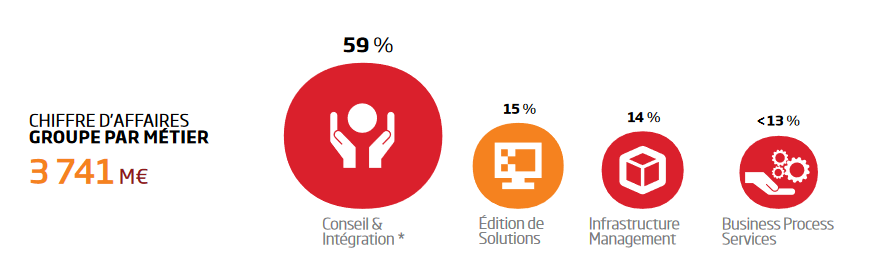
\includegraphics[width=\textwidth,height=\textheight,keepaspectratio]{chiffesClefs.png}
		\caption{Chiffres clefs de l'entreprise.}
		\label{chiffresCles}
	\end{center}
\end{figure}
\newpage
Sopra Steria accompagne les entreprises depuis la définition des stratégies, jusqu’à la réalisation de travaux de consulting en passant par l’intégration de systèmes, le développement de solutions applicatives ainsi que d’outsourcing applicatif. 
Elle combine valeur ajoutée, innovation dans les solutions apportées, qualité industrielle et performance des services délivrés.\\
De cette façon, elle est le partenaire de référence des grandes entreprises et organisations qui recherchent le meilleur usage du numérique pour assurer leur développement et leur compétitivité.\\
Le groupe apporte une réponse globale aux enjeux de développement et de compétitivité des grandes entreprises et organisations.
\smallbreak
\begin{figure}[!hp]
		\begin{center}
			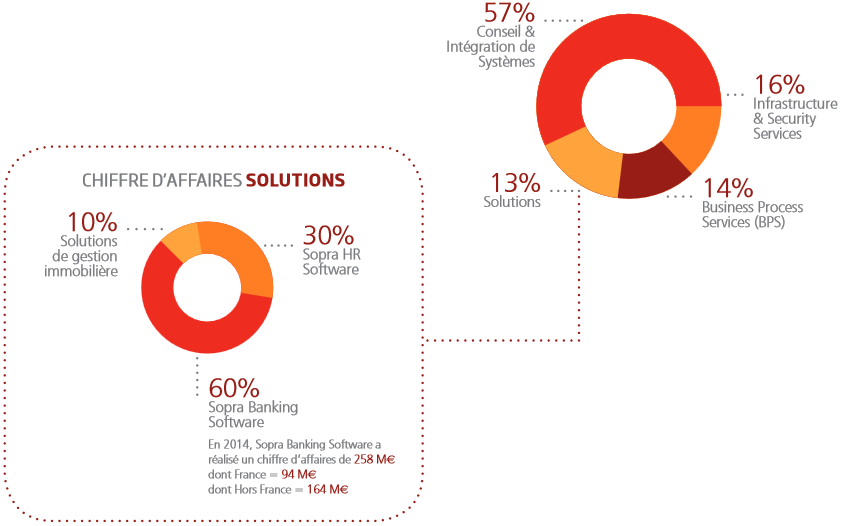
\includegraphics[width=\textwidth,height=\textheight,keepaspectratio]{chiffreClefsMetier.png}
			\caption{Chiffres clefs par métier.}
		\end{center}
\end{figure}
\newpage
\subsection{Diversité des secteurs}
Sopra Steria intervient sur plusieurs secteurs d’activités qui sont divisés en \gls{BU}. La liste exhaustive des secteurs est présentée dans la figure \ref{secteurs}.
\smallbreak
\begin{figure}[H]
	\begin{center}		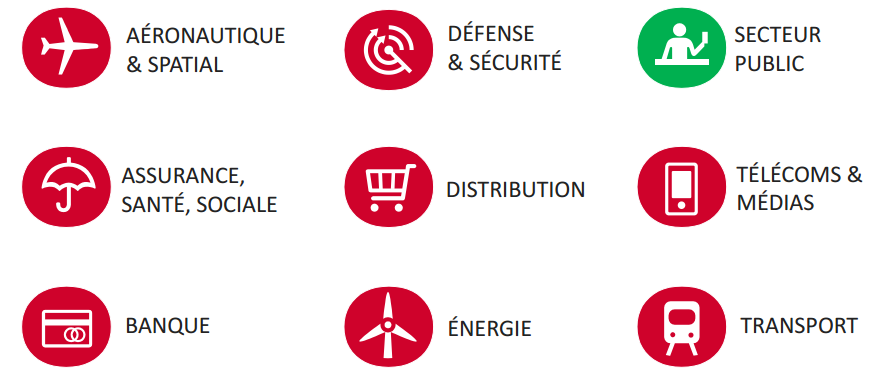
\includegraphics[width=0.80\textwidth,height=0.80\textheight,keepaspectratio]{secteursActivites.png}
		\caption{Activités de Sopra Steria.}
		\label{secteurs}
	\end{center}
\end{figure}
Nous nous intéresserons particulièrement au secteur public qui est celui dans lequel j'ai pu réaliser mon stage et mon apprentissage. La figure \ref{parts} représente les parts des différents secteurs. On observe que le secteur public/défense fait partie des trois pôles les plus rentables.
\smallbreak
\begin{figure}[H]
	\begin{center}	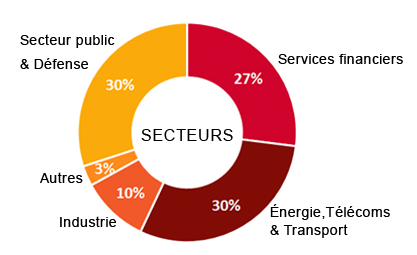
\includegraphics[width=0.7\textwidth,height=0.8\textheight,keepaspectratio]{secteursSopra.png}
		\caption{Parts du secteur public en pourcentage de chiffres d'affaire.}
		\label{parts}
	\end{center}
\end{figure}
\clearpage
\newpage
\subsection{Le secteur public}
Le secteur public est subdivisé en quatre agences dont les différents acteurs sont basés dans de grandes villes françaises et étrangères. Ces agences représentent l'identité du secteur public et possèdent leurs propres clients comme on le voit sur la figure \ref{agences}.
\begin{figure}[H]
	\begin{center}
		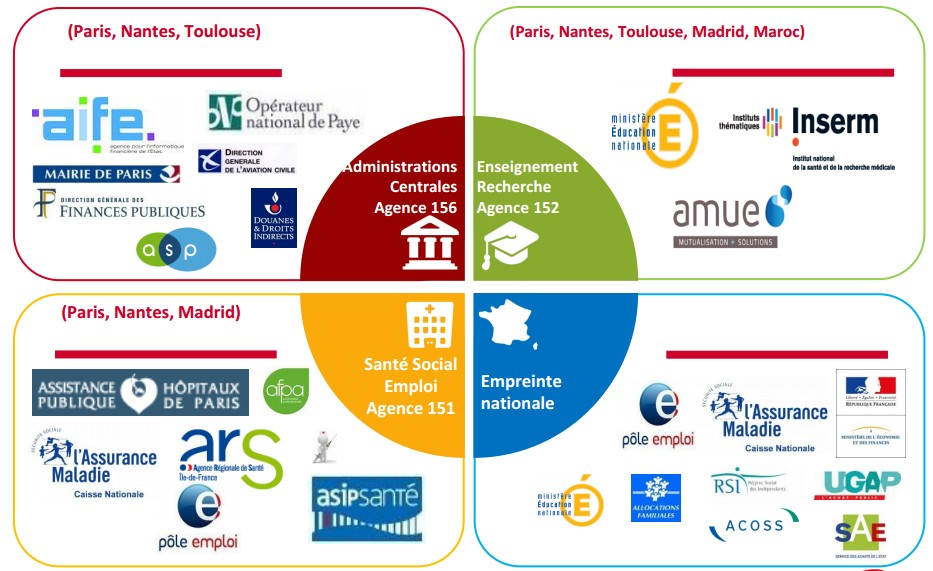
\includegraphics[width=\textwidth,height=\textheight,keepaspectratio]{identiteSecteurPublic.png}
		\caption{Identité du secteur public.}
		\label{agences}
	\end{center}
\end{figure}
J’effectue mon contrat de professionalisation au sein de l'agence 156, dans une équipe déployée chez le client pour le compte de l’AIFE à Noisy-le-Grand (93160 – Seine Saint Denis – France).
\newpage
\clearpage
\section{Contexte du projet Chorus Pro 2017}
Chorus Pro 2017 (logo figure \ref{logoCpp}) est une solution  permettant la dématérialisation fiscale des factures, elle accessible par :
\begin{itemize}
\item un portail web accessible depuis internet,
\item des flux de données en envoyant et en reçcevant des fichiers de données structurées grâce au format \gls{XML},
\item des appels de service web grâce aux \gls{API}.
\end{itemize}
Plus d'un million d'entreprise sont concernées et devront obligatoirement adresser leur facture à Chorus Pro.
\begin{figure}[H]
	\begin{center}
		
\includegraphics[width=0.3\textwidth, height=\textheight, keepaspectratio]{cpp2017.png}
		\caption{Logo de la solution Chorus Portail Pro 2017.}
		\label{logoCpp}
	\end{center}
\end{figure}
\subsection{Présentation du client}
L'AIFE (logo figure \ref{logoAife}) est un service à compétence nationale créé par le décret du 11 Février 2005, dont les missions majeures sont~:
\begin{itemize}
\item piloter l’urbanisation du \gls{SI}\footnote{Un SI représente tous les élements participant à la gestion et à la diffusion de l'information dans une organisation.} financière de l’État ;
\item maintenir en condition opérationnelle le système d’information Chorus, de gestion de la dépense, de la recette non fiscale et de la comptabilité de l’État ;
\item piloter de nouveaux projets interministériels ou ministériels et leur intégration dans le système d’information Chorus ;
\item accompagner le changement dans les ministères et auprès des utilisateurs.
\end{itemize}
\begin{figure}[H]
\begin{center}

\includegraphics[width=0.3\textwidth, height=\textheight, keepaspectratio]{aifedef.png}
\caption{Logo de l'AIFE.}
\label{logoAife}
\end{center}
\end{figure}
\newpage
\subsection{Besoin adressé}
En France, c'est la loi n\degree 2008-776 du 4 août 2008 de modernisation de l'économie qui a introduit la facture au format dématérialisé. Sa mise en œuvre a été fixée au 1er janvier 2012 et cette dématérialisation s’inscrit dans une démarche de rationnalisation et de simplification de l’action publique. Mise dans l'obligation de recevoir les factures électroniques de ses fournisseurs, l'AIFE a déployé le portail "Chorus Factures". Ce dernier assure une transmission normalisée des factures en mode manuel ou en mode flux de données pour les émetteurs déposant un volume de facture important. Ces saisies représentent respectivement des émissions de factures que l'on appelera unitaires et en masse.\\\\
Parallèlement, des chantiers de dématérialisation ont été menés par la \gls{DGFiP} dans le cadre de la modernisation de son système de gestion informatique.
L’ordonnance n\degree 2014-697 du 26 juin 2014 fixe le point de départ d’une nouvelle étape en instaurant une obligation de dématérialisation des factures pour les fournisseurs et une obligation de réception pour les administrations. Elle s'imposera aussi bien à l'État qu'aux collectivités et aux établissements publics, selon des modalités et un calendrier défini.\\\\
Le périmètre total, évalué à 95 millions de factures à l'année, confère au projet un impact réel sur la dépense des entreprises. L'effet levier devrait être conséquent en termes de temps gagné sur toute la chaîne de traitement.\\
Cette même ordonnance prévoit, pour les entreprises fournisseurs de l'État, des collectivités locales et des établissements publics, l'obligation d'adresser leurs factures sous format dématérialisé à partir de 2017. La voie d'un étalement progressif a été préférée à une bascule applicable en une seule fois à toutes les entreprises. Ce choix assure une transition plus aisée, côté fournisseurs, mais aussi une mise en œuvre opérationnelle dès le démarrage pour les administrations. Ainsi, l’obligation sera progressive en fonction de la taille de l'entreprise~: les plus importantes en 2017, les \gls{ETI} en 2018, les \gls{PME} en 2019 et les micro-entreprises en 2020.\\\\
Si le bénéfice sera sans doute important pour les entreprises du système, à terme, l'opération devrait être également bénéfique pour les entités publiques. Ces dernières pourront bénéficier d'un système automatisé de bout en bout, jusqu'à la transmission des mandats et des pièces justificatives.\\
Le choix retenu par l'État va au-delà des orientations fixées par l’Union Européenne. La solution mutualisée Chorus Factures Pro 2017 concerne la facturation des marchés mais également l'ensemble des autres factures fournisseurs de la sphère publique.
\newpage
\subsection{Champ d'application du système}
Le système s'adresse aux fournisseurs de l'État. Ils sont identifiés comme étant les entreprises dont le siège social est établi :
\begin{itemize}
\item en France,
\item en Union Européenne (hors France),
\item hors Union Européenne et hors France,
\item en Polynésie française,
\item en Nouvelle Calédonie,
\item les fournisseurs en cours d’immatriculation,
\item les particuliers,
\end{itemize}
Il est demandé que les factures soient soumises à des destinataires représentés actuellement uniquement par l'État. L'État est représenté sous formes de différentes composantes :
\begin{itemize}
\item les \gls{EPN} : Centre National de la Recherche Scientifique, Pôle Emploi, Chambre de Commerce et d'Industrie;
\item les collectivités territoriales et leurs groupements : villes, métropoles, conseils
régionaux, conseils départementaux;
\item les établissements publics de santé : centres hospitaliers, établissements d'hébergement pour personnes âgées dépendantes;
\item les établissements publics locaux :
\begin{itemize}
\item établissements publics de coopération intercommunale,
\item établissements publics locaux d’enseignement,
\item syndicats mixtes,
\item établissements publics sociaux et médico-sociaux,
\item régies dotées de la personnalité morale, c’est à dire les régies personnalisées,
\item autres catégories d’établissements publics locaux.
\end{itemize}
\end{itemize}
\newpage
L'application Chorus Pro 2017 comprend les fonctionnalités suivantes :
\begin{itemize}
\item la gestion des factures permettant la saisie des factures, leur consultation et le suivi de leur traitement,
\item la consultation des engagements et des bons de commandes émis par les
services de l’état,
\item la conservation de l’ensemble des factures et des pièces jointes pendant 10 ans,
\item la gestion des utilisateurs et l'administration des structures,
\item la gestion des sollicitations apportant de l'aide en cas de difficulté,
\item la mise à disposition d'un portail permettant de tester les interfaces avec Chorus Pro avant leur mise en production appelé portail de Qualification.
\end{itemize}
Elles sont traduites par des interactions utilisateurs/solution dans la figure \ref{schematisation}.
\begin{figure}[H]
	\begin{center}
		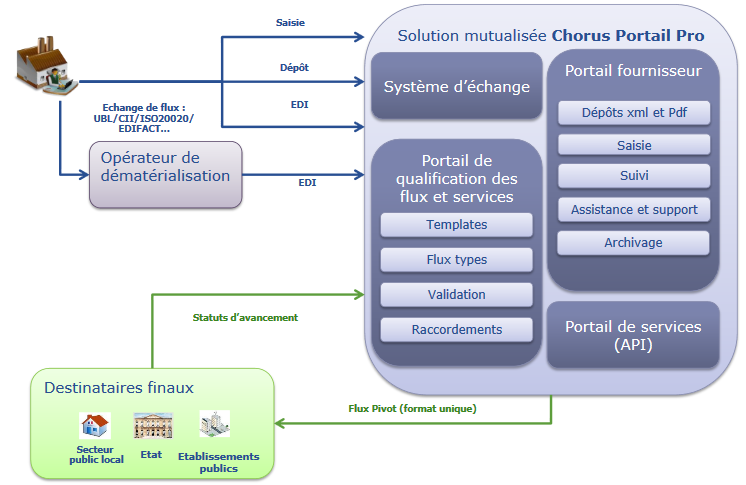
\includegraphics[width=0.8\textwidth,height=\textheight,keepaspectratio]{solutionSimplifiee.png}
		\caption{Schématisation de l'application Chorus Pro.}
		\label{schematisation}
	\end{center}
\end{figure}
\clearpage
\newpage
Ces fonctionnalités sont accessibles par divers moyens pour les émetteurs et les récepteurs de factures. Les fonctionnalités sont synthétisés dans la figure \ref{tableauMoyens}.
\begin{figure}[H]
	\begin{center}
		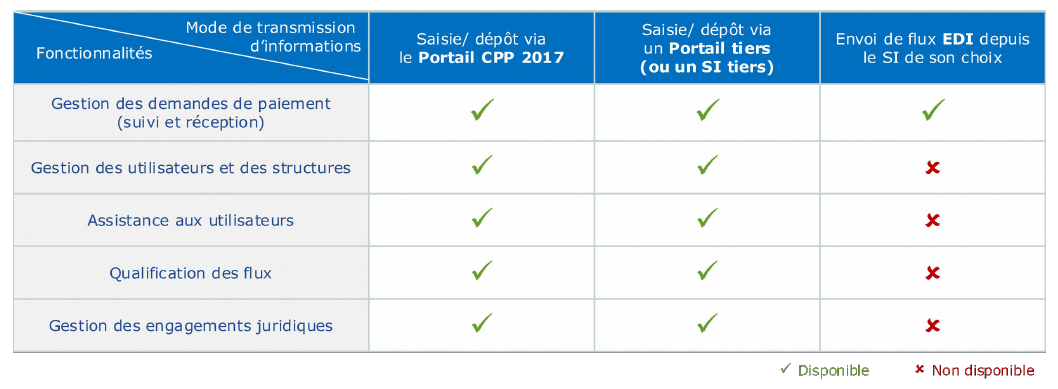
\includegraphics[width=0.7\textwidth,height=\textheight,keepaspectratio]{tableauMoyensFonctionnalites.png}
		\caption{Moyens d'interactions avec l'application Chorus Pro.}
		\label{tableauMoyens}
	\end{center}
\end{figure}
~~\\
\textbf{Mode EDI}
~~\\
Ce canal permet d’échanger de manière automatisée et standardisée des flux de tous les types de factures autrement appelées demandes de paiement. Deux modes d’accès sont possibles sur le canal EDI :
\begin{itemize}
\item Le dépôt en direct : le fournisseur émet lui-même les flux EDI à destination de Chorus Pro 2017,
\item Le dépôt via un concentrateur technique : les demandes de paiement ne sont pas transmises directement par le fournisseur, mais par un tiers ayant pour rôle de prendre en charge la construction et la gestion des flux EDI. 
\end{itemize}
~~\\
\textbf{Mode service}
~~\\
Ce canal permet aux fournisseurs de soumettre des factures et de suivre leur évolution au travers de l'appel de services. Ces services peuvent être consommés par un portail tiers par exemple mis en place par une administration partenaire. Les fonctionnalités offertes par les appels de services sont similaires à celles de la solution web.
~~\\
~~\\
\textbf{Mode portail web}
~~\\
Le portail fournisseur et le portail de qualification : ils offrent aux fournisseurs un site web leur permettant de soumettre des demandes de paiement et de suivre leur évolution. Il offre également aux fournisseurs des fonctionnalités de création et gestion de comptes utilisateurs pour identifier les salariés ou agents du fournisseur à même d’utiliser le système Chorus Pro 2017.
\clearpage
\newpage
\subsection{Contraintes}
La solution du système Chorus Pro est construite de manière à assurer sa pérennité ainsi que sa maintenabilité. Sopra Steria s'est donc engagé à respecter les normes et standards ouverts du marché, de l'AIFE et de l'interministériels. L’architecture applicative et technique du système s’inscrit dans le respect : 
\begin{itemize}
\item	des normes et standards : IP, HTTP, SSL/TLS, XML, Services Web \gls{SOAP} et \gls{REST},
\item	des référentiels généraux assurant la sécurité et l’interopérabilité avec les applicatifs des autres Ministères et partenaires,
\item	des principes et des outils du cadre de cohérence technique.
\end{itemize}
~~\\
Le système Chorus Pro 2017 propose une architecture applicative et évolutive basée sur les standards technologiques \gls{J2EE} dans la recherche de l’ homogénéisation et de la minimisation du nombre de technologies utilisées. Les développements reposent sur un socle applicatif et technologique industriel. Ce socle industriel couvre les phases allant du développement à la production et s’inscrit dans la mouvance de DevOps\footnote{Mouvement dans lequel les équipes de réalisation et d'exploitation travaillent ensemble.} permettant d’automatiser au maximum le passage du développement à la production. Les logiciels libres\footnote{Logiciel dont l'utilisation, la modification ou sa duplication sont permises sans obligations légales.} sont privilégiés dans la définition de la solution, tout en prenant garde qu’ils restent compatibles et dans l’esprit du socle technique de Chorus Pro. Le respect de ces différents éléments permet de faciliter la mise en œuvre et de réduire la complexité et les coûts.\\
La solution Chorus Pro 2017 doit maintenir la qualité de service attendue au fur et à mesure de l’évolution du système. La solution ne doit pas posséder de point de défaillance ou de goulot d'étranglement. Ces contraintes doivent être respectées pendant toute la durée de disponibilité du système soit 99,5\% du temps.\\
Pour répondre à ces problématique l'architecture du système est extensible, élastique et performante. L'amélioration des performances du système est assurée par l'ajout de serveurs virtuels et/ou physiques (\gls{RAM}, \gls{CPU}, disques). On parle alors de scalabilité horizontalle et verticale correspondant respectivement à la possibilité d'ajouter des serveurs et d'upgrader ces derniers.
De plus tous les éléments logiciels, infrastructures matérielles et réseaux du système Chorus Pro 2017 sont redondés et résiliants. Pour assurer la capacité de traitement Chorus Pro offre des mécanismes de répartition de charge sur les différents composants redondés du système et sur la synchronisation et la réplication des données entre les sites d’exploitation. En cas de dysfonctionnement majeur du site principal de production ce système autorise un redémarrage intégral en quelques jours grâce à un \gls{PRA}.  
\newpage
\section{Solution proposée par Sopra Steria}
\subsection{Périmètre du projet}
Nous sommes plus de 100 collaborateurs à travailler sur le projet Chorus Pro. Nous sommes répartis en 7 pôles comme le montre l'organigramme en figure \ref{organigramme}. J'ai intégré le pôle build en réalisant des tâches transverses (communes à plusieurs pôles) pendant la durée de ma formation à Sopra Stéria.\\
Les missions indiquées sur l'organigramme constituent le périmètre du projet couvert par chacun des pôles. Ils assurent du bon déroulement des montées de version et des corrections applicatives de Chorus Pro sur les environnements de production.\\
\begin{figure}[!hp]
		\begin{center}
			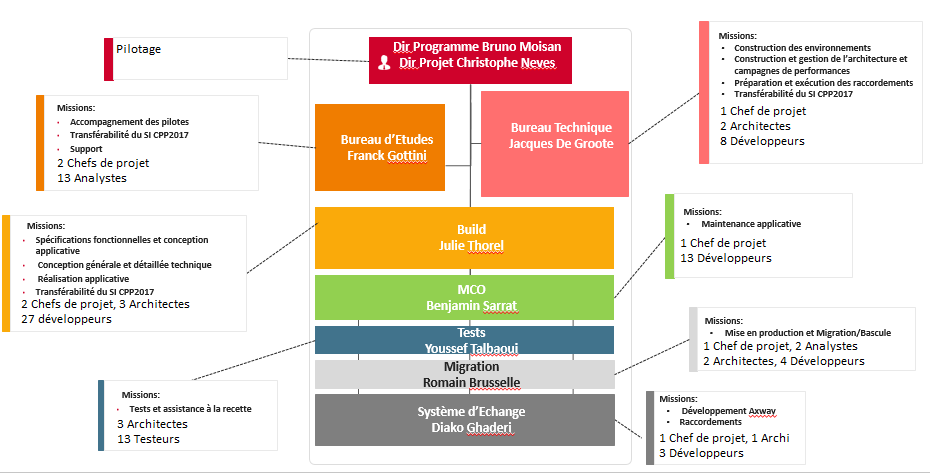
\includegraphics[width=\textwidth,height=\textheight,keepaspectratio]{organigramme.png}
			\caption{Organigramme des pôles du projet Chorus Pro 2017.}
			\label{organigramme}
		\end{center}
\end{figure}
\clearpage
\newpage
La solution Chorus Pro doit assurer la continuité avec une solution existante CPPv1. C'est un système de facturation utilisé par le ministère de la justice et le ministère de l’agriculture, ce système est amené à être englobé par Chorus Pro. A la date du 11 novembre 2017, les utilisateurs de cette plateforme utiliseront Chorus Pro. La figure \ref{friseCpp} explicite le planning de mise en production de Chorus Pro 2017 avec la prise en charge de la migration des données de CPPv1.
\begin{figure}[!hp]
		\begin{center}
			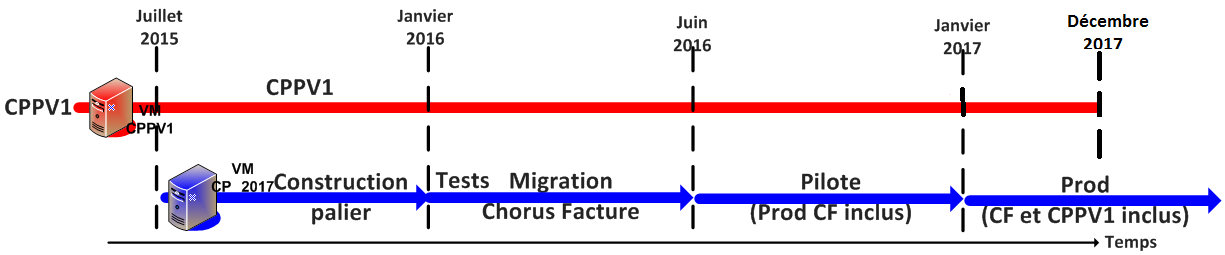
\includegraphics[width=\textwidth,height=\textheight,keepaspectratio]{friseCpp.png}
			\caption{Planning de mise en production et de migration.}
			\label{friseCpp}
		\end{center}
\end{figure}
\subsection{Limites et perspectives}
Chorus Pro s'inscrit dans un contexte novateur dans lequel le système doit évoluer selon les retours utilisateurs partenaires de la solution. Chaque évolution est analysée afin d'en mesurer les impacts fonctionnels puis évaluée techniquement par les équipes de réalisation. Cela permet à nos équipe de proposer une solution technico-fonctionnelle chiffrée en jour-homme.\\
Le groupement Sopra Steria - Capgémini présente des évolutions à forte valeur ajoutée au client dans leur rôle de conseiller. Notre devoir de conseil impose nos équipes à apporter un éclairage de spécialiste quant à la faisabilité de ces nouveaux développements. Le nombre d'évolutions envisagées ne permet pas de réaliser des ateliers de validation dans les temps imposés et leur réalisation ne peuvent pas être prises en compte au même moment. Il est donc important d'avoir une bonne planification pour ne pas impacter toute la chaine de réalisation. Par ailleurs, il faut que les équipes de pilotage s'assurent d'obtenir une charge constante afin de la répartir sur les développeurs dont le nombre ne doit pas fluctuer de manière régulière et en fonction d'un pic de charge.\\ 
\clearpage
\newpage
\subsection{Solution fonctionnelle}
Les sociétés Sopra Steria Group et Capgemini s’associent sous la forme d’un groupement solidaire pour présenter une offre à l’AIFE. Elles sont soutenues dans cette démarche par la société Axway qui interviendra en sous-traitance dans l’exécution de l’opération.\\
Ce groupement apporte à l’AIFE son excellente connaissance du contexte et des méthodes de travail. En effet, il montre une présence continue et historique aux côtés de l’AIFE à travers de nombreuses opérations (de construction et de maintenance) récentes et actuelles.\\
Les deux principes directeurs que nous avons retenus dans la constitution de ce groupement sont les suivants~:
\begin{itemize}
\item quel que soit le champ d’activité projet, les équipes sont intégrées et constituées sur la base des meilleures compétences mobilisées par les membres du groupement,
\item aucun mécanisme de client/fournisseur n’est mis en place au sein du projet, c’est-à-dire qu’aucune des deux sociétés n’est engagée vis-à-vis de l’autre sur un livrable\footnote{Un livrable représente le résultat d'une prestation.} quel qu’il soit.
\end{itemize}
Le planning du projet est ambitieux mais réalisable, le groupement a ainsi conçu un plan de développement en phase avec cette ambition. Au-delà de la capacité à délivrer, la maîtrise du délai passe par~:
\begin{itemize}
\item une capacité commune de décider dans les instances et à faire appliquer les décisions,
\item une anticipation des moyens et une maîtrise des processus pour ôter toute inertie dans le déroulement du projet.
\end{itemize}
\newpage
\clearpage
\section{Architecture du système}
\subsection{Architecture conceptuelle}
\begin{figure}[H]
	\begin{center}
		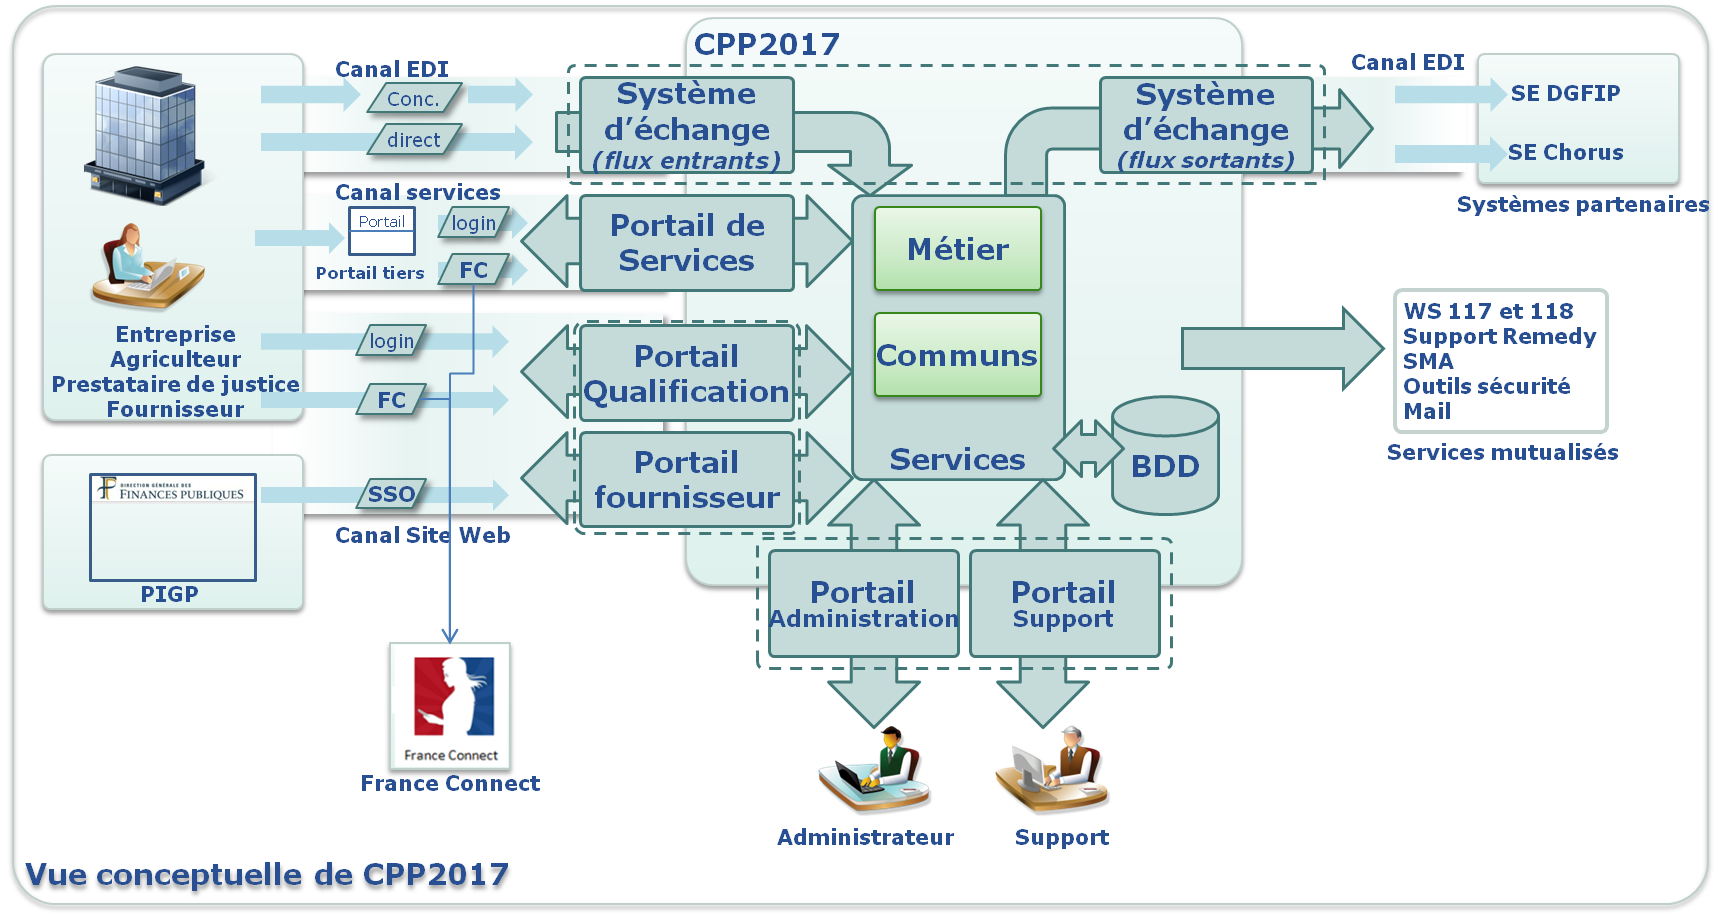
\includegraphics[width=\textwidth, height=\textheight, keepaspectratio]{archiConceptuelle.png}
		\caption{Architecture conceptuelle de Chorus Pro.}
	\end{center}
\end{figure}
Le système Chorus Pro 2017 est mis à la disposition de l’ensemble des fournisseurs et des entités administratives récipiendaires de demandes de paiement. Les fournisseurs peuvent aussi bien être des entreprises privées que des établissements publics. Ce sont des agriculteurs, des prestataires de justice qui effectuent des demandes de paiement au travers de Chorus Pro 2017.
\subsubsection{Les agents administrateurs et le service support}
La gestion opérationnelle du système Chorus Pro 2017 (administration, pilotage et suivi de l’activité, support utilisateurs) est réalisée par des agents ou prestataires de service. Ils se répartissent sur deux types d’activité : 
\begin{itemize}
\item les administrateurs : ils prennent en charge les tâches d’administration applicative et fonctionnelle du système (gestion du contenu éditorial, gestion des référentiels, modification du paramétrage, etc.) ainsi que les tâches liées au pilotage et au suivi de l’activité du système (gestion des alertes et incidents applicatifs et fonctionnel, analyse et suivi statistiques de l’activité),
\item Le service de support : il prend en charge le suivi et la gestion des demandes d’assistance et signalements effectués par les utilisateurs du système Chrous Pro 2017 (i.e. les fournisseurs).
\end{itemize}
\subsubsection{Les systèmes partenaires}
Les systèmes partenaires sont l’ensemble des systèmes prenant en charge l’acheminement des demandes de paiement reçues par le système Chorus Pro 2017 jusqu’aux récipiendaires des demandes de paiement. Deux systèmes partenaires sont identifiés pour le système Chrous Pro 2017 :
\begin{itemize}
\item	Le système d’échange Chorus SE2016\footnote{Plateforme applicative et technique multiservices.},
\item	Le système d’échange DGFIP.
\end{itemize}
\subsubsection{Les services mutualisés}
Les services identifiés, à date, sont : les services WS 117 et 118 pour obtenir des informations de référentiels telles que les numéros de SIREN/SIRET de l’INSEE, les fonctions du module SMA pour réaliser l’archivage et la consultation des documents, les fonctions des outils sécurité, notamment, pour le contrôle des signatures, les fonctions de mail pour les envois des notifications et le système de support remedy pour la gestion de demandes de support ne pouvant être traitées au niveau de Chorus Pro 2017. 
\clearpage
\newpage
\subsection{Architecture applicative}
Ce chapitre décrit les principes et règles mis en œuvre sur le système Chorus Pro 2017 pour identifier et organiser les différents modules applicatifs qui le composent. Ils constitueront un élément de base pour convertir, au fur et à mesure de l’avancée des spécifications fonctionnelles détaillées, les fonctions en services et composants logiciels et les répartir dans les modules applicatifs.\\
L’architecture de la solution Chorus Pro 2017 doit être conçue en cohérence et dans la continuité des travaux d’urbanisation. Les travaux existants doivent être complétés avec une structuration de la vue applicative du SI. Elle permet de rationaliser les composants applicatifs et les référentiels par une urbanisation des services. Il est nécessaire de structurer les domaines applicatifs suivants :
\begin{itemize}
\item	demandes de paiement,
\item	portail,
\item	échanges,
\item	administration,
\item	utilitaire,
\item	sécurité.
\end{itemize}
Pour mettre en œuvre de manière pérenne la construction de la solution Chorus Pro 2017, une première version de la cartographie applicative (cartographie applicatif) a été réalisée. Cette cartographie applicative est un cadre de structuration de la vue applicative. Le schéma de la figure \ref{vueApplicative} présente cette cartographie applicative cible détaillée.\\
\begin{figure}[H]
	\begin{center}
		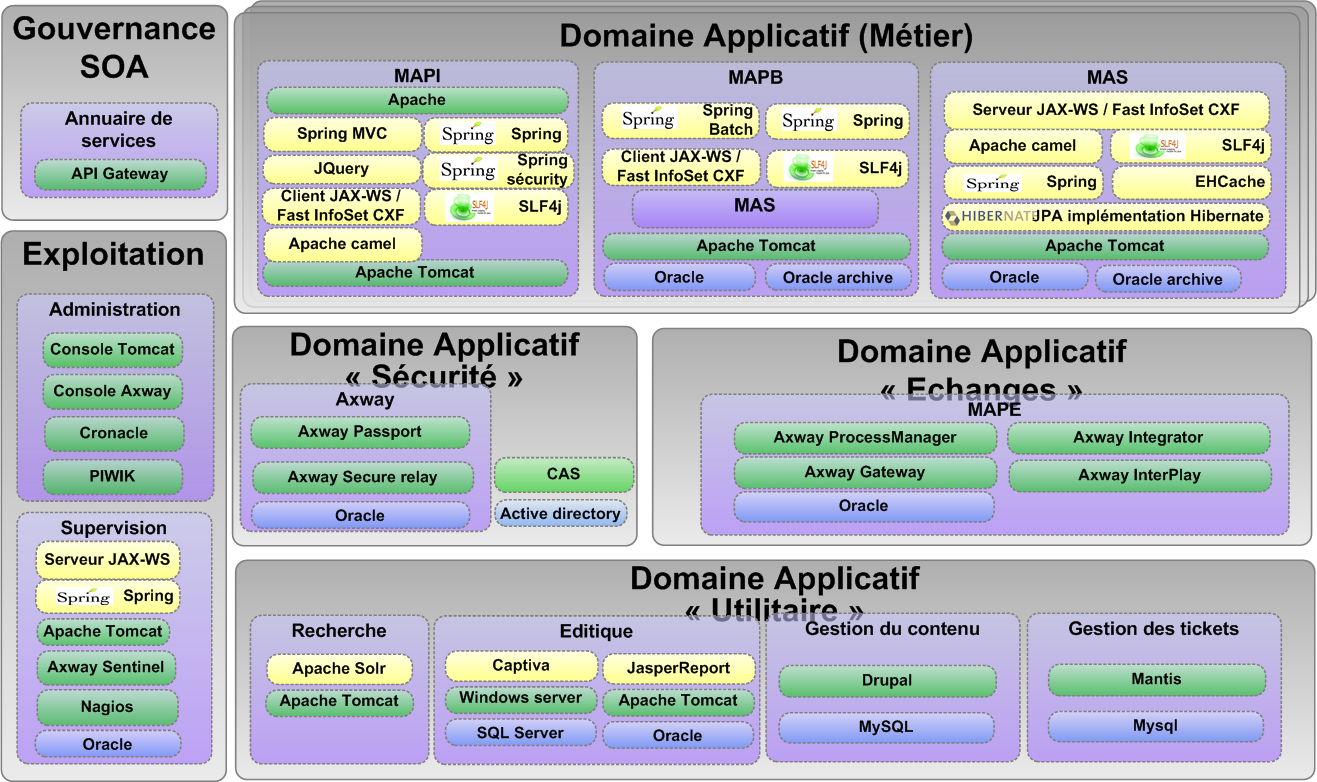
\includegraphics[width=\textwidth, height=\textheight, keepaspectratio]{cartographieApplicative.png}
		\caption{Cartographie applicative du système Chorus Pro.}
		\label{vueApplicative}
	\end{center}
\end{figure}

Cette structuration met au centre du SI le domaine applicatif Demandes de paiement.
Ce domaine s’appuie sur le domaine Utilitaire qui fournit les services mutualisés et transverses suivants :
\begin{itemize}
\item	service de recherche,
\item	notification et émission de courriels,
\item	editique,
\item	données référentielles externes (WS117 et WS118 évoqués précédemment),
\item	service de reconnaissance de caractère : \gls{LAD},\gls{RAD} et \gls{ROC}.
\end{itemize}
Le domaine « échanges » permet d’isoler et de rationaliser les échanges avec les SI externes :
\begin{itemize}
\item	le portail de services,
\item	le portail EDI entrant et sortant.
\end{itemize}
Cette première structuration de la vue applicative permet d’analyser et de cadrer l’ensemble des applications à construire. D’autre part, la vue applicative doit garantir la complétude de la structuration applicative des fonctions du SI issues de la vue fonctionnelle. Cela doit se traduire par l’identification de liens entre les fonctions de la vue fonctionnelle et les modules applicatifs de services de la vue applicative.\\
Un module applicatif (MA) est un regroupement de traitements, il existe deux types de modules applicatifs :
\begin{itemize}
\item les modules applicatifs de pilotage (MAP) implantent un ou plusieurs Cas d’Utilisation de la Vue Fonctionnelle. Ils pilotent les interactions avec les modules applicatifs de services (MAS),\\
\item les modules applicatifs de services (MAS) encapsulent un ensemble cohérent de données métier (silo) et fournissent les services de gestion de ces données en appliquant les règles de gestion associées.
\end{itemize}
\begin{figure}[H]
	\begin{center}
		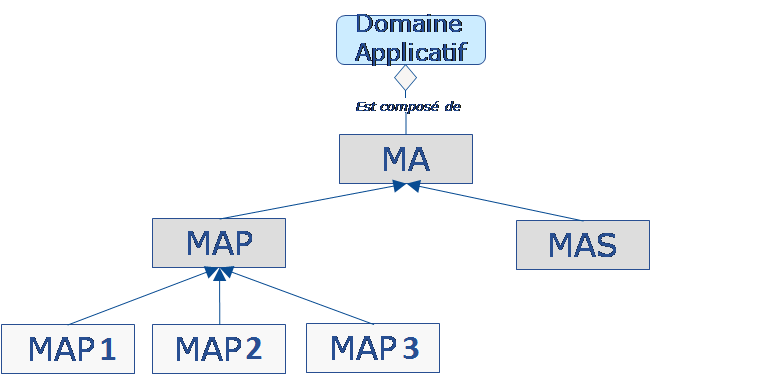
\includegraphics[width=\textwidth, height=\textheight, keepaspectratio]{archiApplicative.png}
		\caption{Architecture applicative.}
	\end{center}
\end{figure}
\clearpage
\newpage
\subsection{Architecture technique}
Les développements spécifiques réalisés dans le cadre du projet Chorus Pro 2017 seront structurés selon le modèle de développement en couches. 
Cette structuration illustrée en figure \ref{couches} s’applique aux Modules Applicatifs de Pilotage (MAP) et aux Modules Applicatifs de Services (MAS) :
\begin{itemize}
\item	les MAP implémentent généralement la couche présentation (ou vue dynamique) mais peuvent aussi utiliser les autres couches pour des services locaux (par exemple un MAPB peut utiliser la couche de persistance pour gérer son état d'avancement)
\item	les MAS utilisent les couches Services, Métier (ou logique métier) et Persistance (Accès aux données) pour implémenter un service
\end{itemize}
\begin{figure}[H]
	\begin{center}
		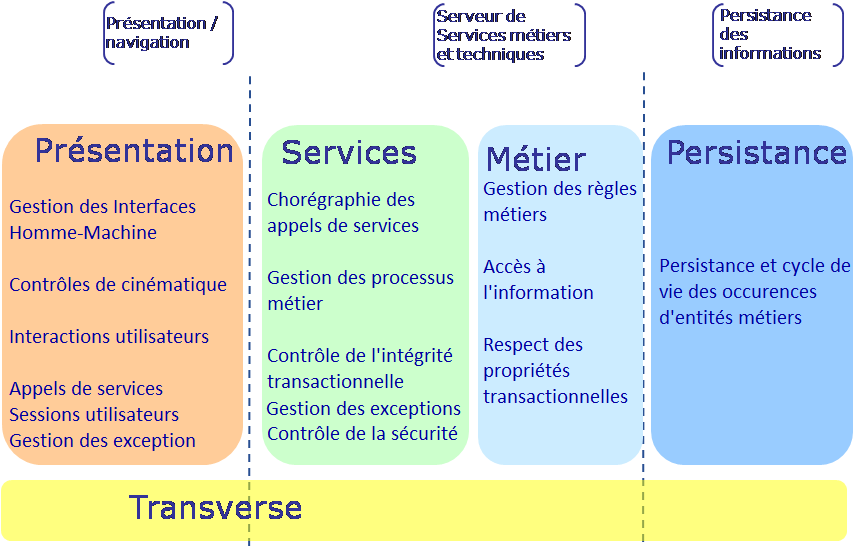
\includegraphics[width=\textwidth, height=\textheight, keepaspectratio]{couchesModules.png}
		\caption{Simplification schématique de l'architecture en couches.}
		\label{couches}
	\end{center}
\end{figure}
\clearpage
\newpage
Le besoin de concevoir les applications en couches découle de la nécessité de les structurer pour en maîtriser le développement. Cette structuration permet :
\begin{itemize}
\item	de maîtriser la complexité des applications. Chaque couche a ses propres responsabilités et utilise la couche située en dessous d’elle,
\item	d’améliorer le découplage entre composants de l’application. Chaque couche peut être développée et testée de manière individuelle,
\item	d’optimiser les temps de développement, par factorisation ,
\item	de normaliser les points d’interaction. Les points d’entrée dans cette architecture sont la couche Présentation (accès Web) et la couche Services (accès via les Services Web).
\end{itemize}
Le passage d’une couche vers une autre doit impérativement se faire via des interfaces qui représentent chacune un service d’accès (introduction de la notion de contrats de services).
La communication s’effectue directement entre les couches adjacentes. Une couche d’un niveau donné ne peut solliciter les services des couches éloignées.
La cohérence entre l’urbanisme (qui conçoit les plans des SI dans une perspective de fonctionnement rationnel et d’évolutivité) et l’architecture d’un projet (qui en construit les blocs applicatifs), est d’autant plus aisée à assurer si l’on parvient à découper les blocs applicatifs selon les couches du modèle de l’architecture applicative logique.
Le fait d’avoir une interface standardisée et normalisée permet de remplacer un composant sans impacter le reste de l’ensemble.
L’impact des évolutions futures de l’application est minimisé par le découplage de l’application (réutilisation plus aisée des méthodes existantes, une modification sur une couche ne nécessite généralement que la modification de la couche supérieure).
\clearpage
\newpage
\subsection{Environnements}
Les composants et fonctionnalités décrits dans les chapitres précédents sont instanciés dans différents environnements dit de « production » ou « projet ».\\
Les environnements « production » concernent l’environnement productif ainsi que tous les environnements générés à partir de celui-ci (environnement de support, de reprise d’activité).\\
La liste des environnements de production, ainsi qu’une description des responsabilités est décrite ci-dessous :
\begin{itemize}
\item	PROD : environnement PRODuctif, sur lesquels les utilisateurs CPP sont connectés (portail de service, portail EDI, portail web utilisateur et administrateur),
\item	PRA : environnement de secours Plan de Reprise d’Activité, permettant la restauration des éléments de PROD en cas d’incident majeur,
\item	PPRD : environnement de PRé-PRoduction, permettant de qualifier les mises en production avant l'exécution en PROD,
\item	SUPP : environnement de SUPPort, copie de la production permettant aux équipes de support de qualifier et reproduire les incidents avec des jeux de donnée les plus récentes,
\item	SUPPRA : environnement de secours Plan de Reprise d’Activité, permettant la restauration des éléments de SUP en cas d’incident majeur,
\item	QLF : environnement de QuaLiFication en self-service de la solution et des flux partenaires,
\item	PERF : environnement d’exécution pour les tests de PERFormances.
\end{itemize}
Il faut noter que les  environnements de PRA et PERF partagent les ressources matérielles d'exécution (serveurs) et ne peuvent être instanciés simultanément.
Les environnements projets sont les environnements liés au développement et aux processus de livraison de la solution par le titulaire: 
\begin{itemize}
\item	DEV : environnement de DEVeloppement et de tests unitaires de la solution,
\item	TST : environnement de TeSTs et de livraison de la solution,
\item	REC : environnement de RECette transverse,
\item	MNT : environnement de MaiNTenance, exécution automatique de tests de non régression\footnote{Bug logiciel où une fonctionnalité ne fonctionne plus correctement ou plus du tout.},
\item	BAS : environnement Bac A Sable permettant de réaliser de POC et autres.
\end{itemize}
\clearpage
\newpage
\section{Ingénierie}
\subsection{Gestion des exigences}
Le but des bonnes pratiques de développement est de produire un code robuste (pas de dérive mémoire, pas de dérive des temps de réponse) et de savoir diagnostiquer les anomalies  afin d'être capable de rétablir les services rapidement.\\
Des exigences ont été définies par les équipes transverses du projet sur la structuration du code, les pattern à respecter ou à proscrire, les points de contention, la scalabilité de l'application et la volumétrie. L'ensemble des exigences sont rappelées aux équipes lors de réunions régulières.\\ Elles concernent :
\begin{itemize}	
\item l'attendu du contenu des couches présentées précédemment,
\item framework et pattern utilisables,
\item dépendance entre les couches : mode de communication, entre chaque couche, responsabilité des couches,
\item réalisation des tests unitaire (doivent couvrir +65\% de la classe),
\item utilisation des bons niveaux de log selon le contexte,
\item documentation des développements complètes,
\item requête sql performantes testées sur environnement,
\item respect des normes de sécurité.
\end{itemize}
\subsection{Gestion des versions}
Les livrables de l'équipe que j'intègre (build) sont des versions de la solution. Chaque version embarque 3 types de contenu :
\begin{itemize}
\item Des anomalies détectées sur les versions précédentes et corrigées pour que l’application fonctionne mieux,
\item De la tranche ferme qui correspond à des fonctionnalités définies dans le cahier des charges,
\item Des évolutions qui sont des fonctionnalités en plus, non prévues dans le cahier des charges.
\end{itemize}
Une trop grande granularité\footnote{La granularité correspond au numéro de version. Il peut varier selon des modifications correctives, évolutives ou autres actions sur le système.} au niveau de la gestion de versions des modules et des services applicatifs entraine une lourdeur de la gestion de la configuration. Une multiplication des versions au niveau MAS entraine un impact trop important sur les MAP.
L’évolution du numéro de version suit les règles suivantes :
\begin{itemize}
\item	La version majeure correspond à des évolutions fonctionnelles majeures ou une refonte très importante du code des composants.
\item	La version mineure est incrémentée lors des intégrations projet ainsi que lors de modification fonctionnelle mineure. A chaque incrémentation de la version majeure, la version mineure est remise à 0. 
\item	La version bugfix est incrémentée uniquement lors de la livraison de correction d’anomalies détectées en phase de recette et suivantes on parle alors d'itération corrective.
\item	La version release est mise à jour uniquement lors de l’intégration palier. Ce numéro de version est purement technique.
\end{itemize}
\clearpage
\newpage
\section{Management de projet}
Chacun des 7 pôles du projet a une équipe de pilotage. L'une de leur mission est le suivi d'activités de tous les membres de leur pôle. 
\subsection{Planification}
Chacun des pôles est partagé en domaines. La figure \ref{domaines} représente la répartition des acteurs selon les domaines dans le pôle build. Les responsables sont chargés de la répartition des tâches sur les ressources disponibles. Ils doivent s'assurer que toutes les tâches relatives à leur domaine peuvent être complétées dans les temps impartis.
\begin{figure}[H]
	\begin{center}
		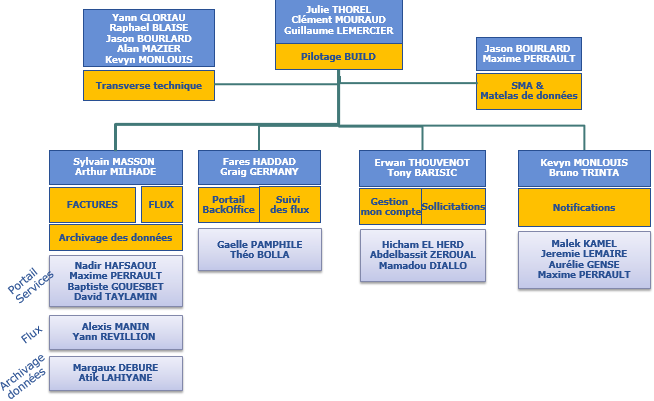
\includegraphics[width=\textwidth,height=\textheight,keepaspectratio]{domaines.png}
		\caption{Domaines du pôle build.}
		\label{domaines}
	\end{center}
\end{figure}
\subsubsection{Suivi d’avancement}
C'est grâce à un plan de charge que les responsables peuvent assurer le suivi d'avancement. Il se présente sous la forme d'un fichier excel dans lequel apparaissent plusieurs informations clefs. La granularité des tâches présentes dans le fichier dépend de la complexité de sa réalisation. Découper une réalisation longue en plusieurs sous tâches permet de diviser le travail sur plusieurs resources si nécessaire. La figure \ref{pdc} est un exemple de plan de charge.
\newpage
On peut  y voir :
\begin{itemize}
\item la ressource : la personne réalisant la tâche,
\item le budget estimé (en jours-hommes)\footnote{Unité de mesure correspondant au travail d’une personne pendant une journée. [wikipédia - 2017]} : chiffrage initial de la tâche,
\item le consommé (en jours) : jours consommé par la resource,
\item le \gls{RAE} (en jours) : l'estimation du nombre de jours restant selon la resource pour compléter la tâche,
\item la dérive : différence entre le consommé + \gls{RAE} et le budget estimé.
\end{itemize}
\begin{figure}[H]
	\begin{center}
		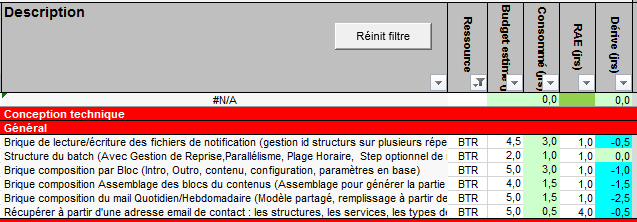
\includegraphics[width=\textwidth,height=\textheight,keepaspectratio]{planDeCharge.png}
		\caption{Plan de charge du chantier notification.}
		\label{pdc}
	\end{center}
\end{figure}
Il y a plusieurs niveau de plan de charge. Le plan de charge niveau projet prend en compte tous les domaines de chacun des pôles et les chantiers transverses. Les plans de charge de pôle sont composés des chantiers\footnote{Un chantier est un ensemble de tâche à réaliser pour la réalisation d'un nouveau développement.} qui les concernent et d'une décomposition plus précises des tâches de ses domaines. Certains chantiers transverses ont leur propre plan de charge afin d'assurer un meilleur suivi des acteurs mobilisés pour sa réalisation.
\subsubsection{Gestion des risques et de la qualité}
Les risques applicatifs sont intrinsèquement liés à la qualité du code. Des standards de qualité du code sont imposés et contrôlés. Une de mes tâches transverses a été de contrôler le bon respect de ces standards. Tous les acteurs du projet sont sensibilisés aux risques et aux engagements pris auprès des clients quant à la qualité du code.\\
Les informations sont partagées lors de plusieurs réunions hebdomadaires et mensuelles. Je réalise aussi un point quotidien sur le domaine sur lequel je suis responsable afin de déterminer l'avancement des tâches attribuées et celles à prévoir. J'assiste à une réunion hebdomadaire dans laquelle sont conviés les acteurs transverses, les responsables de domaine et l'équipe de pilotage du pôle build. Une réunion mensuelle est organisée avec tous les acteurs du projet afin de donner les grandes directions.
\paragraph{Dépassement des temps}
~~\\
Lorsque le chiffrage est réalisé il prend en compte la difficulté de la tâche concernée, le contexte dans lequel elle s'inscrit (besoin d'appréhender des notions transverses,  aborde des nouvelles technologies) mais aussi une contingence. Ce budget est accordé à une ou plusieurs resources pour prendre en compte la réalisation complète de la charge : réalisation, test sur un poste local, test sur un environnement projet. Ce budget peut être ré-évalué lors de la réalisation de la tâche. Si une tâche s'avère plus longue ou fastidieuse qu'intialement prévue il est du devoir de la personne qui réalise la tâche de remonter une alerte au responsable de son domaine afin qu'il prenne les décisions nécessaires.
\paragraph{Manipulations manuelles}
~~\\
Les actions manuelles peuvent représenter un risque et sont toujours réalisées avec précautions. Les procédures automatisées sont préférées. L'automatisation peut intervenir sur tous les pôles du projets. Ainsi des campagnes de tests ont été automatisées afin de réaliser des tests du portail web. Ces tests seront réutilisés en tests de non-régression\footnote{Une régression est une fonctionnalité qui cesse de fonctionner.} et représenteront un gain de temps considérable en plus de limiter le risque de régression. Des scripts de déploiement automatique ont aussi été mis en place. Ces derniers permettent de s'assurer du bon déploiement de tous les composants dans les versions correspondantes et assurent un déploiement rapide.  
\paragraph{Contrôle de la qualité}
~~\\
Des outils open-source sont utilisés pour s'assurer de la qualités du code. 
\begin{itemize}
\item Jenkins : Outil d'intégration continue,
\item Sonar Qube : Outil de mesure de la qualimétrie du code.
\end{itemize}
Jenkins nous permet d'exécuter des jobs sur des machines distantes. On s'assure de la bonne compilation de chacun des dévelopemments réalisés grâce à un job lançant une compilation maven à intervalle régulier. Ce même job lance une analyse Sonar Qube du code source.\\
Sonar Qube possède des indicateurs qui sont représentés par une lettre allant de A à E. Une de mes tâches transverses est de m'assurer du respect des règles définies dans Sonar Qube. Pour réaliser cette tâche je réalise un support que je présente aux réunions hebdomadaires aux responsables de domaines afin que ceux-ci puisse avoir une vision globale des règles les plus violées. J'ai aussi présenté un support lors d'une réunion mensuelle afin de sensibiliser tous les acteurs du projet à ces règles de bonne conduite applicative.
\subsection{Conduite du changement}
La conduite du changement est un sujet majeur dans ce projet qui mobilise un grand nombre de collaborateurs. Le changement passe par une bonne communication entre les différentes composantes du projet. Toute démarche d'amélioration constructive est encouragée.\\
Dans le cadre de mes responsabilités transverses j'adresse des mails de bonnes pratiques applicatives dans un objectif de meilleures performances, maintenabilité ou respect des règles sonar.
Des mesures plus légères peuvent améliorer la rigueur dans le code. J'ai notamment pu mettre en place un module sur le Jenkins \emph{Continuous Game} avec l'aide d'un architecte du projet. Ce module est un système à points réalisant un classement. Des points sont marqués en participant à une compilation réussie. En revanche des points sont retirés aux personnes ayant contribué à une compilation non fonctionnelle.
\clearpage
\newpage
\section{Challenges et accomplissement}
Mon expérience de plus d'un an sur le projet m'a permis de monter en compétence sur des sujets fonctionnels et techniques du projet Chorus Pro. Je me suis d'abord positionné en tant que responsable adjoint puis responsable d'un domaine me permettant d'aborder des notions de gestion d'équipe :
\begin{itemize}
\item la répartition des tâches,
\item le suivi d'avancement,
\item le suivi de la qualité.
\end{itemize}
De part mon ambition et ma curiosité professionnelle j'ai pu prendre en charge des tâches transverses concernant la gestion de la qualité du code fourni mais aussi le partage des bonnes pratiques. Mon implication dans ses tâches m'a permis d'apprendre à communiquer avec nos équipes notamment en réalisant des supports à destination des développeurs. Je travaille régulièrement sur de nouveaux supports dans le but d'améliorer la sécurité applicative et les performances de l'application (respect des standards de sécurité, optimisation des requêtes SQL).\\
Ces différentes actions m'ont permis d'étendre mon réseau de connaissances au sein de l'entreprise et de m'impliquer davantage dans divers projets de Sopra Steria, me permettant ainsi, de comprendre l'activité générale et la politique du groupe. Ainsi j'ai participé activement, en interne, à un projet qui propose aujourd'hui aux collaborateurs d'avoir accès à différents retours d'expériences, leur permettant ainsi de mieux comprendre les actions, conséquences et erreurs ou réussites à reproduire ou à éviter dans leurs futures missions.
\newpage
\section{Analyse critique}
Le bon déroulement du projet est observable grâce aux trois axes suivants :
\begin{itemize}
\item le respect des processus,
\item la bonne communication,
\item le partage d'une même vision.
\end{itemize}
Beaucoup de processus sont mis en place pour améliorer et optimiser les échanges entre les différents pôles. Ces processus sont essentiels au bon déroulement du projet. Ils permettent d'obtenir plus de clareté, d'organisation et de temps. J'appuierai mon argumentation sur le processus de traitement d'une anomalie décrit sur la figure \ref{cycleVieAnomalie}.\\
Comme on le voit, ce processus fait intervenir 3 acteurs différents : Le client, le pôle de test, le pôle du build. 
\begin{figure}[!hp]
		\begin{center}
			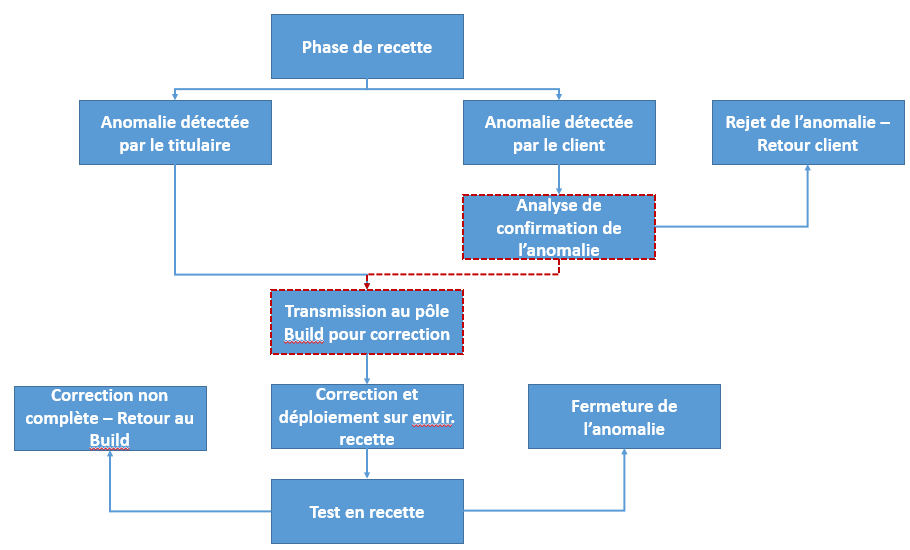
\includegraphics[width=1.1\textwidth,keepaspectratio]{cycleAnomalie2.png}
			\caption{Cycle de vie d'une anomalie.}
			\label{cycleVieAnomalie}
		\end{center}
\end{figure}
\clearpage
\newpage
Ce processus permet de stabiliser des versions en recette avant de les mettre en production et d'organiser le travail des développeurs. Un stock important d'anomalies signifie que des développements correctifs auront lieu dans les versions suivantes de l'application.\\
En un an près de 10 000 anomalies ont été créées par les titulaires (Groupe Sopra Steria - Capgemini) ou par le client. Pour chacune d'entre elles, une analyse a eu lieu dans les équipes de tests à la suite de quoi une majorité des anomalies sont retransmises au build. Je porte mon intérêt à ce moment précis du processus et aux moyens par lesquels une amélioration pourrait y être apporté.\\
A ce moment là c'est aux équipes du build d'apporter une analyse du problème applicatif et d'en apporter une correction dans le cas nominal. D'autres cas sont à envisager :
\begin{itemize}
\item l'anomalie est un faux positif car elle est issue d'un problème de jeux de données verrolé ou n'est pas avérée,
\item l'anomalie est une évolution de l'application et doit donc être traitée par le bureau d'études du projet pour validation,
\item l'anomalie est un doublon d'une anomalie déjà existante, voire déjà corrigée.
\end{itemize} 
Dans les cas énumérés c'est un retour aux équipes de tests pour une nouvelle analyse. L'intérêt de la revue de ce processus est de limiter le nombre d'échanges non productifs entre les deux pôles. On peut exploiter les retours d'expérience de testeurs et des développeurs en organisant des réunions permettant un échange sur l'origine des anomalies relatives aux jeux de données, mieux cadrer le processus de renseignement des anomalies lors d'une transmission ou encore modifier le fonctionnement d'une des briques du processus.\\
Ces réflexions peuvent être portées sur de nombreux processus. Le projet évolue en ce sens au fil des observations remontés lors des points réguliers entre les différents pôles. Il serait intéressant de considérer les processus les plus lourds pour identifier les bénéfices que cela pourrait apporter au fonctionnement des équipes sur le projet.
\begin{comment}
Les anomalies ont une gravité :
\begin{itemize}
\item bloquante signifiant qu'une fonctionnalité a disparu ou n'existe pas,
\item importante traduisant qu'une fonctionnalité ne remplit pas 
\item moyenne n'impactant pas le fonctionnement de l'application mais gênant 
\item basse  nécessitant un ajustement.
\end{itemize}
\end{comment}
\clearpage
\newpage
\section{Bilan}
Ce contrat de professionalisation m'a beaucoup apporté. J'ai pu monter en compétence sur des domaines qui m'étaient jusqu'alors très peu accessibles. Les échanges avec les équipes m'ont aussi formé pour les démarches administratives et le fonctionnement en entreprise. Les responsabilités qui m'ont été confiées par mes différents responsables, que je remercie une fois de plus, m'ont permis de prendre des initiatives avec confiance. Cela m'a amené à faire preuve d'un professionnalisme que je n'avais jamais pu adopter auparavant.\\
Ce projet ambitieux nécessite une forte implication et conscience professionnelle. Elles permettent de réaliser les développements nécessaires dans les temps impartis malgré le retard que le projet avait intialiement pris. Il est parfois nécessaire de corriger des anomalies bloquantes avant une livraison en production tout en tenant compte des jalons sur des développements correctifs en parallèle.\\
Le fait d'évoluer dans un environnement aussi riche et diversifié est une chance. L'équipe est composée de nombreux profils : experts, intermédiaires et débutants. Les échanges n'en sont que plus enrichissants, tous les acteurs apprennent des autres et l'entraide est naturelle.
L'uniformité du code grâce aux normes de développement que nous respectons permet de plus facilement s'adapter aux tâches qui nous sont confiées.
La documentation, les commentaires, et la bonne structuration du code est indispensable. Nous devons pouvoir fournir du code maintenable facilement et durablement.
\newpage
\clearpage
\section{Conclusion}
Je suis très satisfait d’avoir effectué mon stage ainsi que mon alternance dans l'entrepise Sopra Stéria car cela m’a permis de vivre une forte expérience du travail en entreprise. Grâce à cette formation, j’ai pu m’enrichir énormément autant sur le plan technique que sur le plan humain.\\
J’ai découvert le travail au sein d'une grande équipe qui est un réel atout et à la fois une contrainte forte. La diversité des profils et la densité des équipes favorisent l'entraide entre les collaborateurs tout en obligeant d'obéir à une certaine rigueur dans la mesure où le travail d'une personne importe à de nombreux autres collaborateurs. J’ai donc redoublé de vigilance lors de l’exécution de mes tâche se en essayant de me fixer des objectifs Spécifiques, Mesurables, Acceptables, Réalistes et Temporellement définis (SMART).\\
J'ai réussi à progresser techniquement sur des technologies nouvelles et des framework spécifiques me permettant d'accéder à des positions de responsables sur des domaines. J'ai donc pu me familiariser avec les notions de gestion d'équipe notamment concernant la répartition des tâches ainsi que la gestion des risques. Grâce aux conseils de mon tuteur et des autres collaborateurs j'ai pu prendre des initiatives et me positionner sur des tâches représentant un challenge pour moi comme la réalisation de points technique ou la rédaction d'une conception technique d'un chantier. \\
La bonne humeur au sein du projet m'a permis de faire de magnifiques rencontres malgré l’urgence des livraisons. Le contexte de mon alternance a largement dépassé mes attentes et a enrichi mes compétences professionnelles. J'ai pu mettre en pratique des aspects de l'informatique dans des situations auxquelles je n'avais jamais été confronté.
Cette année, mon stage a confirmé l'importance du travail en équipe et de conditions de travail optimales au profit des objectifs fixés.

\paragraph{Conclusion}
~~\\\\
\[NOUVELLE-TRADUCTION-INCOMING\]
Doing this internship at Sopra Steria was very satisfying for me. I lived a very strong professional experience in this company. Thanks to this internship, I improved a lot in a technical level as much as in a human level. I also discovered big team work which is a huge advantage because every member of the team help each other to make the project progress. It helped me being more thorough in my developments because an inexpert modification may affect the work of many co-workers. I had to focus more on the execution of my tasks.

I learned how to use JAVA EE technology which is essential for web applications development in a company. Every concept approached that i didn’t understand were explained when needed. Thanks to my tutor and the team programmers’ advices, I learned how to use those technologies. The constant project’s teamwork good mood enabled me to make great contacts despite the delivery emergency. In this way, my internship’s conditions exceeded what i was expecting and it improved my professional skills. I had the chance to put informatics aspect into practice in situations that I have never been used to. This year, my internship reinforced the importance of team work and good  conditions in order to fulfill our goals.
\newpage
\clearpage
\appendix
\renewcommand
\listfigurename{Résumé des figures.}
\listoffigures
\newpage
\makeatletter
\renewcommand\@biblabel[1]{\textbullet}
\makeatother
\nocite{*}
\bibliographystyle{plain}
\bibliography{dixitsbiblio}
\end{document}